\chapter{Literature Review}
\label{chap:literature_review}

This chapter briefly describes three projects
(Argus~\cite{argus_end_to_end_service_anomaly_detection_and_localization_from_an_isps_point_of_view},
NetNorad~\cite{netnorad}
and CEM~\cite{crowdsourcing_service_level_network_event_monitoring})
that use end-to-end QoS to localize faults in computer networks.

\section{Argus}

In~\cite{argus_end_to_end_service_anomaly_detection_and_localization_from_an_isps_point_of_view}
is presented Argus, a system to
detect and localize problems in \gls*{isp}'s networks. To achieve this goal, Argus uses
network global information, and also passively collected data from the \gls*{isp}'s
viewpoint to infer
end-to-end QoS, such as traffic to/from end-users to estimate achievable
download
speed~\cite{speed_testing_without_speed_tests_estimating_achievable_download_speed_from_passive_measurements}.

The system's analytics pipeline is illustrated in
Figure~\ref{fig:argus_pipeline}.

\begin{figure}[H]
    \centering
    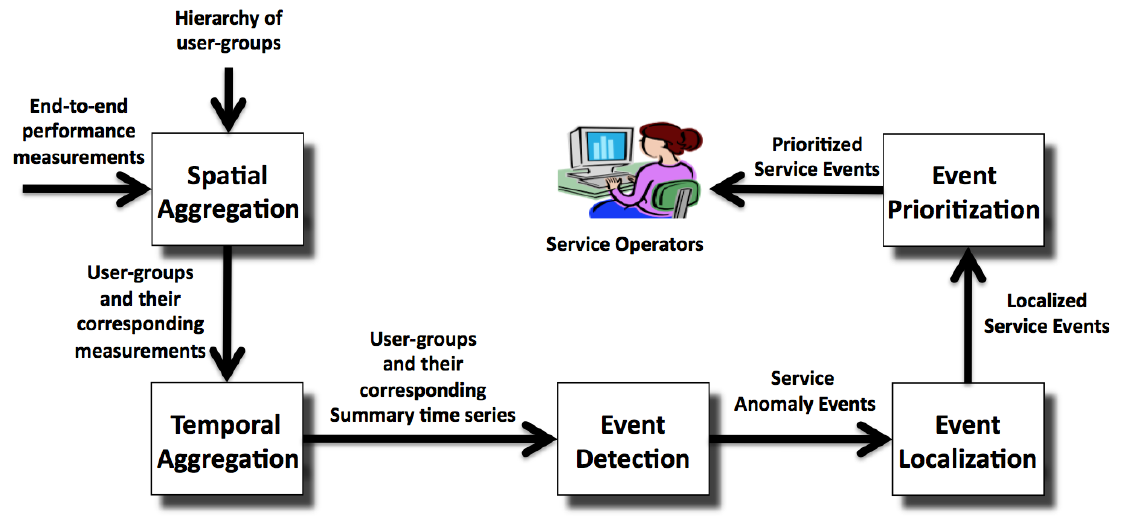
\includegraphics[width=0.8\textwidth]{./figures/literature_review/argus_pipeline.png}
    \caption{Argus pipeline.~\cite{argus_end_to_end_service_anomaly_detection_and_localization_from_an_isps_point_of_view}}
\label{fig:argus_pipeline}
\end{figure}%

The analysis starts with the Spatial Aggregation procedure, in which
end-users are clustered into user-groups. This step improves the system's
scalability, since avoids keeping track the performance of all
individual end-users.
Each user-group is characterized by a set of end-users that share some common
attributes, such as AS or BGP prefix. The used features imposes the possible
fault locations to be inferred.
An example of a spatial aggregation is depicted in
Figure~\ref{fig:argus_spatial_aggregation}.

\begin{figure}[H]
    \centering
    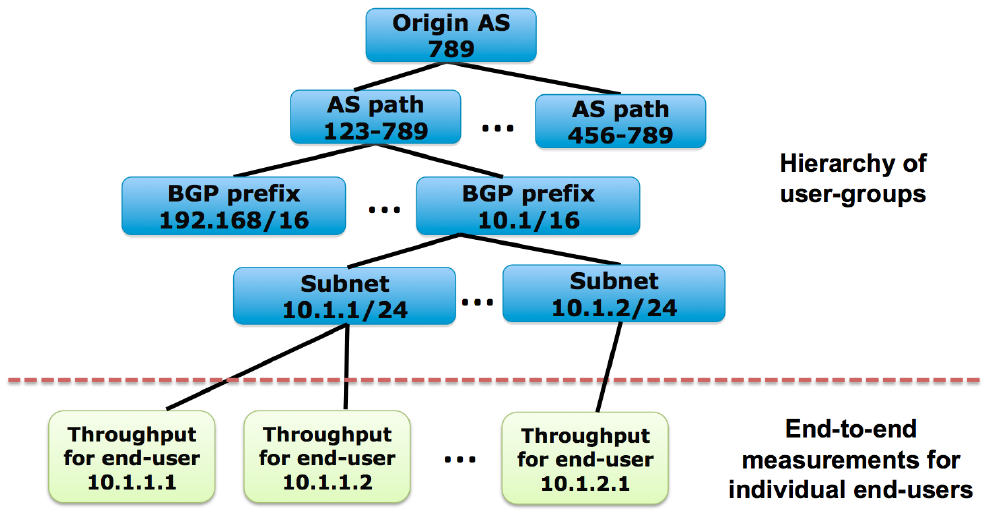
\includegraphics[width=0.8\textwidth]{./figures/literature_review/argus_spatial_aggregation.png}
    \caption{Argus spatial aggregation.~\cite{argus_end_to_end_service_anomaly_detection_and_localization_from_an_isps_point_of_view}}
\label{fig:argus_spatial_aggregation}
\end{figure}%

The Temporal Aggregation phase determines how data
from different end-users of an end-group are combined.
For each user-group, the
measurements of all end-users are grouped in time-bins, and for each
time-bin a summary statistic, such as median or mean, is selected.
Each type of fault can be better tracked by a specific statistic.
As an example, the
minimum of the RTTs can capture the physical propagation delay,
while the average can be related with network congestion. Argus uses median
as the default transformation, since it was empirically identified as
effective to track network flaws, and also robust to individual
end-users variability caused by their local infrastructure.

The Event Detection procedure identifies anomalies in the
summary time series. Argus uses a Holt-Winters variation,  which consists of
an online
method with low run time and memory complexities.

The responsibility of the Event Localization step is to infer fault locations
using spatial and events times correlations.
However, the detailed description of how this
process is implemented was not published.

Finally, the detected problems are sorted according with
their significance, which considers metrics obtained
through the event detection
algorithm, and also the number of affected end-users.

Argus was evaluated using RTT measurements of a CDN hosted in a tier-1 \gls*{isp}\@.
During an one month, 2909 anomalous events were detected.
In general, lower level user-groups were more responsible
for those events than the higher level groups,
and only a small fraction of the end-users caused the end-group anomaly.
Also, 90\% of the events lasted for
at most 1 hour, which was the used time-bin granularity.

Although not investigated by the Argus's authors, the fact that only a
small number
of end-users are responsible for the end-groups events, is an indication that
fault localization can achieve higher precision
with finer spatial aggregation granularity. Besides, the system accuracy was
not studied.

\section{NetNorad}

NetNorad~\cite{netnorad} consists of a Facebook's internal project to
automate the analysis of faults in the Facebook's
network. Previous deployed techniques by Facebook exhibit several
disadvantages, for instance,
human-driven investigation may take hours. Also, cases known as gray failures
cannot be detected only collecting devices information through SNMP or command
line
interface. For example, some devices cannot report it's own malfunctioning, or
some problems can be related with the global network structure.

Facebook's network is structured hierarchically. At the
lowest level there are servers in racks, which are organized in
clusters. A set of clusters in the same building and attached to
the same network characterize a data center. Data centers are grouped
through a network that interconnects them within the same region, and appends
to the Facebook global backbone. Figure
~\ref{fig:netnorad_network_architecture} presents an example of this
architecture.

\begin{figure}[H]
    \centering
    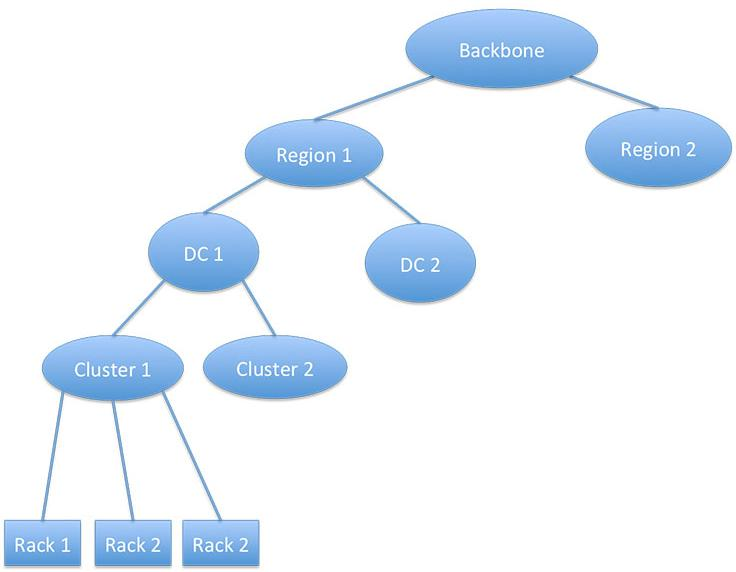
\includegraphics[width=0.7\textwidth]{./figures/literature_review/netnorad_network_architecture.jpg}
    \caption{Facebook's network architecture.~\cite{netnorad}}
\label{fig:netnorad_network_architecture}
\end{figure}%

Unlike Argus, NetNorad uses active probing to assess loss and RTT statistics.
Facebook's servers ping each other, in which
a pinger sends UDP packets to responders, and the latter
send the packets back. The process happens in turns, each pinger
sends packets to all targets, collects the responses, and then repeats
the procedure. A small number of pingers are placed in each cluster,
and the responders are
deployed on all machines. All pingers share a target list, which includes
at least two machines of every rack.

As with Argus, NetNorad applies spatial aggregation techniques.
The pingers group the responses of machines that belong to the same cluster
during a round, and tags them according with their relative location.
Tags are defined by the following patterns:
``DC'' if the target cluster is in the pinger's data center;
``Region'' if the target cluster is outside the pinger's
data center but within the same region;
``Global'' if the target cluster is outside the pinger's
region.

With the tagging process, each cluster have three time series reflecting
different spatial viewpoints, which are tracked through
distinct percentiles over 10-minute
intervals, enabling a fault mitigation reasoning.
For instance, a packet loss spike at the
50th percentile means that probably there is a failure affecting the majority of
machines, while a peak at the 90th and not at 50th
percentile can indicate a small fraction of anomalous servers.
For each combination of proximity tag and percentile is defined two
thresholds, one for trigger and another for clear an alarm.

Considering the three tags, if a high loss is detected in a cluster,
then the fault is probably located at the cluster's data center.
Also, if all clusters in a data center identify a QoS degradation,
then the fault is likely to be placed a layer above the clusters.
Although these simple inferences can reduce the set of possible fault locations,
they are unable to exactly isolate them.
However, a Facebook tool called fbtracert
can improve this analysis, exploring multiple
paths between two endpoints, and checking the
packet loss levels at every hop. Nonetheless, fbtracert exhibits several
limitations.

When automatic investigation is unable to find the failure, then there
is a human involvement to find it. A detailed accuracy analysis is not
presented, however, the infrastructure allows alarms to be raised about 30
seconds far from the network events.

\section{CEM}

In~\cite{crowdsourcing_service_level_network_event_monitoring} is proposed a
framework called Crowdsourcing Event Monitoring (CEM), in which a
monitoring software that runs inside or alongside applications is placed at the
end-hosts, enabling the detection of service level events within seconds or
minutes.

In CEM, each end-host passively collects performance metrics related with a
specific service, such as a VOD application.
Through these data, and to increase the system's scalability,
the end-host itself identifies local problems as
potential network events, and pushes them to a distributed storage to further
analysis.
The framework doesn't specifies how events should be detected,
however, they must be associated with service level problems.

To spatially isolate network flaws, locally detected events and spatial
information are centrally correlated.
The first subproblem of this step is to check if concurrent events
of different end-users are caused by a
network fault. There are several reasons to different hosts identify
simultaneous events not caused by the network.
For example, a high volume of requests in a web service can impact the end-hosts
service performance. Also, it is
possible that simultaneous events occur only by chance, for instance, users
can suffer signal interference on separate wireless routers.
Therefore, through service specific dependencies and the empirical rate of
simultaneous
events, CEM provides a statistical model to determine if
concurrent problems are a coincidence.
In this model, the confidence of a network fault increases with the
number of hosts that detect the event, and also with the number of affected
metrics.
The detailed method indicating how to realize spatial and temporal
correlations to
localize problems is not specified.

CEM was deployed and evaluated in a P2P system, using traces
collected
from users of the Ono plugin in the Vuze BitTorrent client. The system's
output was contrasted with \glspl*{isp} public available reports. In general,
CEM provides a high level system abstraction, lacking several
important deployment issues.
